\documentclass[a4,8pt]{article}
\usepackage[margin=3cm,includefoot]{geometry}
\usepackage{siunitx}
\usepackage{fancyhdr}
\usepackage{tikz}
	\usetikzlibrary{arrows,shapes,positioning,calc,decorations.pathmorphing,patterns}
\usepackage[font=it]{caption}
\usepackage{amsmath}
\usepackage{float}

\pagestyle{fancy}
\lfoot{\sc Charlie Haddon}

\title{Fundamental Particles}
\author{Charlie Haddon}
\pagenumbering{arabic}

\begin{document}

\section{Hadrons}
Inside the nuclei of atoms are neutrons and protons, collectively known as nucleons. These 
particles are also composed of smaller particles which as far as we know are fundamental. 
These particles are called quarks.

\begin{figure}[H]
\begin{center}
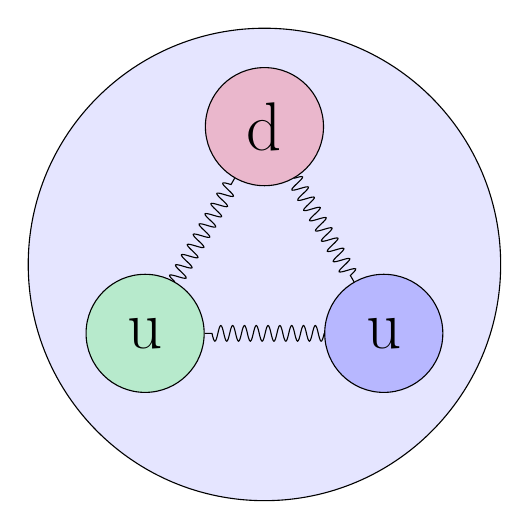
\begin{tikzpicture}
    \draw[fill=blue, fill opacity=0.1] (0,0) circle (3);
    
    \tikzset{every node/.style={draw,circle,inner sep=0pt,minimum size=1.5cm,fill opacity=0.2,
            text opacity=1}}
    \node[fill=red  ] at (90 :1.75) (d ) {\Huge d};
    \node[fill=green] at (210:1.75) (u1) {\Huge u};
    \node[fill=blue ] at (330:1.75) (u2) {\Huge u};

    \draw[decoration={coil,aspect=0,amplitude=1mm,segment length=1.5mm},decorate] (d ) -- (u2);
    \draw[decoration={coil,aspect=0,amplitude=1mm,segment length=1.5mm},decorate] (u2) -- (u1);
    \draw[decoration={coil,aspect=0,amplitude=1mm,segment length=1.5mm},decorate] (u1) -- (d );
\end{tikzpicture}
\caption{An illustration of quarks within a proton}
\end{center}
\end{figure}

\subsection{Quarks}
The aforementioned quarks, up and down, make up the first generation and are the least massive 
and most stable of the quarks. The second generation includes charm and strange quarks and
the third has top and bottom quarks. The masses and instability of quarks are increased for
higher generations. All quarks have corresponding antiquarks with equal mass and opposite 
charge.

\begin{center}
\begin{tabular}[H]{l|l r l r}
Generation 1 & Up/Antiup       & ($u$/$\bar{u}$) & Down/Antidown        & ($d$/$\bar{d}$)\\
Generation 2 & Charm/Anticharm & ($c$/$\bar{c}$) & Strange/Antistrange  & ($s$/$\bar{s}$)\\
Generation 3 & Top/Antitop     & ($t$/$\bar{t}$) & Bottom/Antibottom    & ($b$/$\bar{b}$)\\
\end{tabular}
\end{center}

Quarks of generations two and three quickly decay into generation one quarks.

\subsection{Baryons}
Baryons are a type of hadron that consist of three quarks, similarly, antibaryons consist of
three antiquarks. The most common of these are protons and neutrons. 

\end{document}
